\documentclass[letterpaper]{article}
\usepackage[ngerman]{babel} % Sprache festlegen
\usepackage[utf8]{inputenc}
\usepackage[top=1.2in, left=1.4in, bottom=1.2in, right=1.4in]{geometry} % Seitenränder
%\usepackage{amsmath,amsthm,amssymb} % Mathematische Symbole
\usepackage{url} % Schöne URLs erstellen
\usepackage{csquotes} %Korrekte Gänsefüßchen
\usepackage[onehalfspacing]{setspace} % Zeilenabstand
%\newcommand{\nochOffen}[1]{ \begin{quote} \textbf{Offen:} #1 \end{quote}}
\usepackage{tabularx}
%\newcolumntype{L}[1]{>{\raggedright \arraybackslash}p{#1}}
%\usepackage{biblatex}
\usepackage{graphicx}


\begin{document}

\begin{titlepage}
    \begin{center}
        \vspace*{2cm}
            
        \LARGE
        \textbf{SDG\,in\,Veröffentlichungen\,des\\
        Bundesministermiums\,für\,Forschung\,und\,Entwicklung\,}\\
            \text{Eine Distant Reading Analyse mittels Machine Learning}
            
        \vspace{0.5cm}
        \large
        Seminar \textit{Aktuelle Trends der Informatik}
            
        \vspace{3.0cm}
        
        \normalsize{\textbf{Veronika Marie Heuten}}\\
        \normalsize{v.heuten@studserv.uni-leipzig.de}\\
        \normalsize{Matrikelnr. 3724542}\\
            
           \vspace{3cm}


        24.02.2022
        
        \vspace{0.8cm}
            
        
\includegraphics[width=0.3\textwidth]{img/lpzg_icon.jpg}
          
        \vspace{0.8cm}
        
        \normalsize
        Sommersemester 2021\\
        \vspace{0.8cm}
        \small Betreuung Uni Leipzig: Prof. Dr. Hans-Gert Gräbe\\
        \small Fakultät für Mathematik und Informatik\\
        \small Universität Leipzig\\
            
    \end{center}
\end{titlepage}

\clearpage 
\tableofcontents
\clearpage

\section{Einleitung}
Noch immer leben Menschen in Armut, hungern, haben keinen Zugang zu sauberem Trinkwasser und arbeiten unter menschenunwürdigen Bedingungen. Ein Großteil dieser Probleme resultiert aus der Art, wie wir Menschen leben, miteinander aber auch mit der Umwelt umgehen und welche Hierarchien als selbstverständlich angesehen werden. Diese sind durch Ungleichheit zwischen Geschlechtern, Nationen und Gesellschaftsschichten, die der Mensch im Laufe seines Bestehens selbst hervorgebracht hat, entstanden. Viele dieser Missstände bedingen sich gegenseitig und verschlimmern einander. So geht Armut beispielsweise mit dem unzureichenden Zugang zu Trinkwasser einher, was wiederum hygienische Missstände verursacht und Krankheiten begünstigt. Kranke Menschen wiederum können nur schwer einer Arbeit nachgehen, was wiederum auch Armut und Hunger zur Folge hat.\\
Die Vereinten Nationen haben es sich seit den 1990er Jahren unter der Hilfe verschiedener Initiativen zur Aufgabe gemacht, diese Missstände gemeinsam zu beheben. Aktuell wird diese Mission durch die 17 Sustainable Development Goals (SDG), die es bis 2030 zu erreichen gilt, vorangetrieben. Eines der wichtigsten Mittel, diese Ziele umzusetzen ist Bildung, die möglichst viele Menschen erreicht. Ein Ansatz Bildung möglichst vielen Menschen zugänglich zu machen wird durch Initiative \textit{Education for Sustainable Development} (ESD) vorangetrieben. In Deutschland wird diese durch den \textit{Nationalen Aktionsplan Bildung für nachhaltige Entwicklung} (BNE) umgesetzt. Wie der Aktionsplan BNE die Umsetzung der 17 SDGs gestaltet, soll in dieser Arbeit näher untersucht werden. Für die vorliegende Arbeit werden alle Publikationen des BNE, dessen Vorsitz das Bundesministerium für Bildung und Forschung innehat, mittels Distant Reading Techniken untersucht. Da sich Distant Reading für eine erste Analyse einer großen Menge an Text eignet, wird so versucht heraus zu finden, ob die 17 SDGs im Einzelnen thematisiert werden, ohne jeden Text einzeln lesen zu müssen.\\
Zunächst wird ein kurzer Überblick über die Entstehungsgeschichte der Sustainable Development Goals, ihren Inhalt und die Verbindung von BNE und SDG gegeben. Im Anschluss daran soll erläutert werden, wie in dieser Analyse vorgegangen wird und welche Methoden verwendet werden. Dann folgt eine Beschreibung des verwendeten Datensatzes und wie mit diesem verfahren wird. Im nächsten Abschnitt werden die Ergebnisse präsentiert und anschließend interpretiert. Im abschließenden Teil wird das Vorgehen der Analyse reflektiert und ein Fazit gezogen. 

\clearpage

\section{Sustainable Development Goals und Bildung nachhaltige Entwicklung}
Im Jahr 2000 verständigten sich die Vereinten Nationen auf dem Millennium-Gipfel in New York dazu, den elementaren Problemen der Menschheit gemeinschaftlich entgegenzuwirken. Daraufhin wurden die sogenannten \textit{Millennium Development Goals} (MDG) verabschiedet \cite{BMZ}. In diesen wurden acht Ziele festgelegt, die bis zum Jahr 2015 erreicht werden sollten. Diese Ziele wurden wie folgt definiert: 

\begin{enumerate}
    \item den Anteil der Weltbevölkerung, der unter extremer Armut und Hunger leidet, halbieren
    \item allen Kindern eine Grundschulausbildung ermöglichen
    \item die Gleichstellung der Geschlechter und die Rechte von Frauen fördern
    \item die Kindersterblichkeit verringern
    \item die Gesundheit der Mütter verbessern
    \item HIV/Aids, Malaria und andere übertragbare Krankheiten bekämpfen
    \item den Schutz der Umwelt verbessern
    \item eine weltweite Entwicklungspartnerschaft aufbauen
\end{enumerate}\\
Durch diese ehrgeizigen und bis dahin in der Geschichte einmaligen Ziele konnten sich in den 15 Jahren des Geltungszeitraumes der MDGs mehr als eine Milliarde Menschen aus extremer Armut befreit, Hunger abgebaut, und so vielen Mädchen und Frauen wie nie zuvor eine Schulbildung ermöglicht werden. Jedoch wurden diese Ziele bis zum Jahr 2015 nicht erreicht, was den UN-Generalsekretär Ban Ki-Moon dazu brachte, eine "Post-2015-Entwicklungsagenda", die diese Ziele weiter vorantreiben soll, zu fordern\cite{UN}.\\
In der Tradition der MDGs wurde im September 2015 die \textit{Agenda 2030 für nachhaltige Entwicklung} mit den 17 darin enthaltenen SDGs verabschiedet. Diese Ziele sind die erste internationale Übereinkunft, die das Prinzip der Nachhaltigkeit mit der Bekämpfung von Hunger und Armut miteinander in Beziehung setzt\cite{BMZ}. Die Vereinten Nationen haben es sich zur Aufgabe gemacht, eine sozial, ökonomisch und ökologisch gerechte Welt bis 2030 zu erreichen.\\
Die 17 Ziele lauten in ihren Überschriften: \cite{Agenda2030}
 \begin{enumerate}
     \item keine Armut
     \item kein Hunger 
     \item Gesundheit und Wohlergehen 
     \item hochwertige Bildung 
     \item Geschlechtergerechtigkeit 
     \item sauberes Wasser und Sanitäreinrichtungen 
     \item Bezahlbare und sauberer Energie 
     \item Menschenwürdige Arbeit und Wirtschaftswachstum 
     \item Industrie, Innovation und Infrastruktur
     \item weniger Ungleichheit (in und zwischen Ländern)
     \item nachhaltige Städte und Gemeinden
     \item nachhaltiger Konsum und Produktion 
     \item Maßnahmen zum Klimaschutz
     \item Leben unter Wasser (erhalten und nachhaltig nutzen)
     \item Leben an Land (schützen, wiederherstellen)
     \item Frieden, Gerechtigkeit und starke Institutionen 
     \item Partnerschaften zur Erreichung der Ziele
    
 \end{enumerate}\\
Diese 17 Ziele lassen sich in fünf, etwas gröberer Handlungsfelder zusammenfassen: \textbf{Mensch} (People) , \textbf{Planet} (Planet), \textbf{Wohlstand}, (Prosperity), \textbf{Frieden} (Peace) und \textbf{Partnerschaft} (Parntership).\\
Auch wenn in den letzten Jahren Fortschritte gemacht wurden, wurde das Erreichen der Ziele durch die Coronapandemie weit zurückgeworfen. Darunter leiden besonders die ärmsten Länder\cite{Agenda2030}. Im September 2019 wurde festgestellt, dass die Entwicklungsziele mit der bisherigen Strategie bis 2030 nicht erreicht werden können. Um dies auszugleichen und die SDGs doch noch in ihrem Geltungszeitrum zu verwirklichen, müsste die Weltgemeinschaft jährlich zusätzlich 4,5 Billionen Euro investieren. Besonders durch die weltweite pandemische Lage wurde den Vereinten Nationen vor Augen geführt, dass zur Bewältigung von globalen Herausforderungen nachhaltiges Handeln von besonderer Wichtigkeit ist\cite{Bericht}. Nachhaltiges Handeln kann nur von Menschen umgesetzt werden, die über entsprechendes Wissen verfügen. Durch Bildung zum Thema Nachhaltigkeit werden Bürger*innen die Fähigkeiten an die Hand gegeben, vorausschauend zu denken, interdisziplinäres Wissen zu verinnerlichen, autonom zu handeln und an gesellschaftlichen Entscheidungsprozessen zu partizipieren\cite{BNE}\\
Um die 17 Nachhaltigkeitsziele zu erreichen, bedarf es eines Prozesses des Umdenkens, der auf einer gesamtgesellschaftlichen Ebene vollzogen wird. Aus diesem Grund sehen die Vereinten Nationen den Schlüssel zu einer erfolgreichen Umsetzung der SDGs in Bildung. Das SDG 4 \textit{Hochwertige Bildung} ist dem zu Folge nicht nur eines von vielen Zielen, sondern gleichzeitig auch noch das wichtigste Werkzeug alle Ziele bis 2030 zu erreichen\cite{ESD}.
Im Jahr 1992 wurde mit der Initiative \textit{Education for Sustainable Development} (ESD) ein Aktionsplan geschaffen, der damals zur Umsetzung der Agenda 21\footnote{Die Agenda 21 wurde im Juni 1992 in Rio de Janeiro verabschiedet. Sie enthält klare Ziele und definiert Probleme, die bis zu Beginn des 21. Jahrhunderts behoben werden sollten\cite{Agenda21}} helfen sollte und in dieser Tradition nun für die SDGs bereitsteht. ESD soll dazu beitragen, dass Entscheidungen und die darauf folgenden Handlungen eines jeden Individuums unter Beachtung der jeweiligen Konsequenzen getroffen werden. Um diese Konsequenzen einordnen und erkennen zu können, müssen Individuen über politische, kulturelle, umwelttechnische und soziale Umstände Bescheid wissen und diese einordnen können. In Deutschland wird dies durch den nationalen Aktionsplan Bildung für nachhaltige Entwicklung (BNE) verwirklicht. Dieser Aktionsplan teilt Bildung in verschiedene Bildungsbereiche ein. Diese sind frühkindliche Bildung, Schule, berufliche Bildung, Hochschule,  non-formale/informelle Bildung und Bildung auf kommunaler Ebene\cite{G}. BNE gibt Handreichungen für Lehrende und informiert über Aktionen und Fortschritte im Bereich Nachhaltigkeit.
 
\section{Praktisches Vorgehen}
Mittels Distant Reading wird in dieser Arbeit untersucht, inwiefern die 17 SGDs in den Publikationstexten über den Aktionsplan \textit{Bildung nachhaltiger Entwicklung} automatisch identifzierbar sind. Distant Reading bezeichnet eine quantitative Untersuchung von großen Mengen an Textdaten. Hierbei werden zum Beispiel Worthäufigkeiten oder Kookurrenzen interpretiert. Dies steht im Gegensatz zur Methode des Close Readings, worunter man die herkömmliche inhaltliche Interpretation von Texten versteht\cite{Moretti}.

\subsection{Ansatz des Topic Modellings}
Die Methode des Topic Modeling erstellt für eine Sammlung von Texten oder innerhalb eines einzelnen Textes verschiedene \textit{Topics} [auf Deutsch: \textit{Überschriften}]. Diese Topics setzen sich aus einer Reihe von Worten zusammen, die häufig zusammen auftauchen. Hier wird alleine aufgrund der Häufigkeit, mit der die Worte gemeinsam auftauchen, davon ausgegangen, dass diese in thematischem Bezug zueinander stehen. Die Topics werden aus den analysierten Texten heraus gefunden und benötigen keine externen Wörterbücher oder Trainingsdatensätze. 

\subsection{Verwendete Daten und Vorgehen}
Um der Forschungsfrage nachzugehen, wie die 17 Ziele der nachhaltigen Entwicklung im nationalen Aktionsplan BNE behandelt werden, werden wie bereits beschrieben alle Publikationen des Bundesministeriums für Bildung und Forschung als Datengrundlage verwendet. Alle Publikationen des BNE-Forums werden heruntergeladen und ergeben den Korpus\footnote{Die Texte sind hier zu finden: \\ https://www.bne-portal.de/SiteGlobals/Forms/bne/publikationen/suche\_formular.html?nn=162408}.\\
Um alle Texte als Korpus verwenden zu können, müssen diese im Vorhinein überarbeitet werden. Zunächst werden alle Texte in Kleinschreibung umgewandelt, um ein einheitliches Schriftbild zu erhalten. Im zweiten Schritt werden Stoppwörter entfernt. Stoppwörter sind Worte, die sehr häufig auftreten und keinen Informationsgewinn für das Ergebnis bedeuten. Solche Listen können vorgefertigt verwendet und individuell ergänzt werden. In der vorliegenden Analyse wird die deutsche Stoppwortliste des Phython nltk Packages verwendet. 
Danach werden alle Satzzeichen und Zahlen aus dem Korpus entfernt sowie die Worte lemmatisiert. Für die Lemmatisierung wird der Hannover Tagger (HanTa)\cite{HanTa} herangezogen. Bei der Lemmatisierung wird jedes Wort des Korpus in seine Grundform umgewandelt. So wird zum Beispiel aus dem Wort \textit{nachhaltigkeitsthemen} das Wort \textit{nachhaltigkeitsthema}.\\
Um die Topics aus dem Korpus zu gewinnen, wird MALLET verwendet. MALLET ist ein Java basiertes Package, das mit dem Little Mallet Wrapper auch für Python verfügbar ist. Das MAchine Learning LanguagE Toolkit wurde von Andrew McCallum entwickelt. Er lehrt an der University of Massachusets Amherst\cite{MALLET}\cite{MALLET_WELSH}.\\
Das MALLET Topic Modeling ist LDA basiert. LDA steht für \textit{Latent Dirichlet Allocation}, hierbei handelt es sich um ein im Jahr 2000 vorgestelltes Wahrscheinlichkeitsmodell. Die betrachteten Worte aus den zu verarbeitenden Texten werden gruppiert und ergeben die Topics \cite{LDA}. Die Idee hinter LDA ist, verschiedene Topics in mehreren Dokumenten auszumachen und die Wahrscheinlichkeit dafür zu bekommen, wie stark ein Topic mit einem Dokument zusammen hängt. Da besonders längere Texte dazu neigen Themen zu behandeln, ist es nicht sinnvoll ein Topic pro Dokument zu erhalten. Bei dieser Methode kann herausgefunden werden, welche Topics in den Dokumenten behandelt werden und zudem lässt sich eine Aussage darüber treffen, welche Dokumente eine hohe Wahrscheinlichkeit haben, die gleichen Topics beinhalten\cite{LDAorig}. \\
Im folgenden Modell werden für den Korpus 17 Topics generiert, um im Idealfall ein 1:1 Matching mit den 17 SDGs zu bekommen.\\
Die gewonnenen Topics werden dann betrachtet, und durch Ermessen der Autorin den SDGs zugeordnet. Die Benennung von Topics aufgrund ihres Inhaltes durch die durchführenden Forscher*innen ist bei ungelabelten Topics gängige Praxis\cite{Ramage}.
\clearpage

\section{Ergebnisse}
Der verwendete BNE-Korpus setzt sich aus 35 Dokumenten zusammen. Jedes dieser Dokumente hat im Schnitt 10417 Worte. Der gesamte Korpus hat einen Wortschatzumfang von 35201 Worten. Im Folgenden werden nun die erhaltenen Topics aufgeführt und die am ehesten übereinstimmenden SDG dazu geschrieben. Sollten andere, nicht von einem SDGs abgedeckten Themen erkennbar sein, werden diese ebenfalls aufgeführt. Sind mindestens drei Wörter zu einem Thema vorhanden, wird dieses ausgewiesen. 

\subsection{Topic Modeling BNE-Korpus}

    \textbf{Topic 0} \\
'nachhaltig', \textbf{'entwicklung'}, \textbf{'bildung'}, 'mensch', 'leben', 'unesco', 'mehr', 'welt', 'handeln', 'land', 'kultur', '\textbf{wissen'}, 'müssen', 'weltweit', 'sozial', 'eigen', 'deutsch', 'gehen', 'politisch', 'heute' \\
\textbf{Zugehörige SDG:} 4. Hochwertige Bildung \\
\textbf{Sonstige Themen:} --\\

\textbf{Topic 1} \\
'unesco', 'deutsch', 'deutschland', \textbf{'kulturell'}, \textbf{'kultur'}, 'vielfalt', 'kommission', 'bildung', 'inklusive', 'fördern', \textbf{'immateriell'}, \textbf{'kulturweit'}, 'international', 'biosphärenreservat', 'erhalten', 'global', 'erbe', 'zielen', \textbf{'kulturerbe'}, \textbf{'welterbe'} \\
\textbf{Zugehörige SDG:} - \\
\textbf{Sonstige Themen:} Kultur und kulturelles Leben\\

\textbf{Topic 2}  \\
'hhaltig', 'hsc', 'nac', 'hulen', 'hen', 'demokratie', 'ntw', 'klung', 'haf', 'ung', 'keit', 'ildung', 'lebensform', 'lung', 'orsc', 'isc', 'ild', 'hung', 'international', 'freiheit' \\
\textbf{Zugehörige SDG:} --\\
\textbf{Sonstige Themen:} --\\

\textbf{Topic 3}  \\
'netzwerk', 'stärken', \textbf{'jugendlich'}, 'kommune', 'haus', 'unesco', 'struktur', \textbf{'arbeit'}, \textbf{'prof'}, 'ausgezeichnet', \textbf{'gymnasium'}, 'stadt', \textbf{'schule'}, 'thüringen', \textbf{'universität'}, 'auszeichnung', 'gelsenkirchen', 'herausforderung', 'klimahaus', 'bayern' \\
\textbf{Zugehörige SDG:} 4. Hochwertige Bildung\\
\textbf{Sonstige Themen} Lokaler Bezug\\
  
\textbf{Topic 4} \\
'dekade', 'bne', 'unesco', 'bildung', \textbf{'nachhaltig'}, 'entwicklung', \textbf{'deutschland'}, 'deutsch', 'werden', 'rund', 'projekt', 'tisch', \textbf{'kommune'}, 'aktivität', \textbf{'bonn'}, 'jahr', \textbf{'nationalkomitee'}, \textbf{'kommission'}, 'offiziell', 'auszeichnung'  \\
\textbf{Zugehörige SDG:} 11. Nachhaltige Städte und Gemeinden\\
\textbf{Sonstige Themen:} --\\
    
\textbf{Topic 5} \\
'nachhaltigkeit', 'unesco', 'heute', 'politik', 'entwicklungsland', \textbf{'wachstum'}, 'konvention', \textbf{'erfolgreich'}, 'begriff', 'leitbild', \textbf{'ressource'}, 'staat', 'gemeingut', 'vereint', 'initiative', 'nation', 'schutz', \textbf{'konsum'}, 'bmu', \textbf{'wohlstand'} \\
 \textbf{Zugehörige SDG:} 8. Nachhaltig wirtschaften als Chance für alle \\
 \textbf{Sonstige Themen:} --\\
 
\textbf{Topic 6} \\
\textbf{'vielfalt'}, \textbf{'biologisch'}, \textbf{'natur'}, \textbf{'nachhaltig'}, \textbf{'nutzung'}, 'vgl', 'schutz', 'kasten', 'sowie', 'info', \textbf{'wald'}, \textbf{'mensch'}, 'global', 'kind', \textbf{'lebensraum'}, 'jugendlich', 'konsum', 'art', \textbf{'ökologisch'}, \textbf{'urban'} \\
\textbf{Zugehörige SDG:} 15. Leben an Land \\
\textbf{Sonstige Themen:} --\\

\textbf{Topic 7} \\
'entwicklung', 'indikator', 'nachhaltig', \textbf{'bildung'}, 'werden', 'deutsch', \textbf{'forschung'}, \textbf{'hochschule'}, 'quantitativ', 'datum', 'sowie', 'politisch', 'entsprechend', 'bereich', \textbf{'bildungsbericht'}, 'bundesland', 'hinsichtlich', 'unece', 'qualitativ', 'ergebnis'  \\
\textbf{Zugehörige SDG:} 4. Hochwertige Bildung weltweit\\
\textbf{Sonstige Themen:} --\\

\textbf{Topic 8} \\
'projekt', 'dekade', 'bne', 'entwicklung', 'nachhaltig', 'laufend', 'ergebnis', 'bildung', 'verbreitung', 'nap', 'maßnahme', 'eher', 'lassen', 'zahl', 'vgl', 'aktivität', 'verankerung', 'abgeschlossen', 'transfer', 'eigen'  \\
\textbf{Zugehörige SDG:} --\\
\textbf{Sonstige Themen:} --\\

\textbf{Topic 9} \\
\textbf{'bildung'}, \textbf{'entwicklung'}, 'nachhaltig', 'bne', 'nachhaltigkeit', 'akteur', 'sowie', 'deutsch', 'global', 'engagement', 'umsetzung', 'maßnahme', 'sollen', \textbf{'forschung'}, \textbf{'förderung'}, \textbf{'fördern'}, '\textbf{beruflich'}, 'unterstützen', \textbf{'vernetzung'}, 'struktur' \\
\textbf{Zugehörige SDG:} 4. Hochwertige Bildung weltweit\\
\textbf{Sonstige Themen:} --\\

\textbf{Topic 10} \\
\textbf{'hochschule'}, 'nachhaltig', \textbf{'universität'}, 'nachhaltigkeit', 'entwicklung', \textbf{'studierend'}, \textbf{'forschung'}, \textbf{'netzwerk'}, \textbf{'lehren'}, 'netzwerks', 'www', \textbf{'interdisziplinär'}, \textbf{'uni'}, 'sowie', \textbf{'leuphana'}, 'berlin', \textbf{'wissenschaft'}, \textbf{'studiengang'}, \textbf{'nachhaltigkeitsforschung'}, 'praxis'\\
   \textbf{Zugehörige SDG:} 4. Hochwertige Bildung weltweit \\
   \textbf{Sonstige Themen:} --\\
   
\textbf{Topic 11} \\
'bne', 'ziel', \textbf{'hochschule'}, 'handlungsfeld', 'national', 'kommune', \textbf{'schule'}, 'land', 'iii', 'formal', \textbf{'fachforum'}, 'non', 'aktionsplan', 'commitment', \textbf{'fördern'}, 'rahmen', 'bmbf', 'bund', 'unesco', 'umsetzung' \\
   \textbf{Zugehörige SDG:} 4. Hochwertige Bildung weltweit\\
   \textbf{Sonstige Themen:} --\\
   
\textbf{Topic 12} \\
 'the', 'and', 'education', 'development', 'sustainable', 'that', 'bildung', 'are', 'this', 'entwicklung', 'nachhaltig', 'with', 'berlin', 'germany', 'have', 'not', 'decade', 'national', 'all', 'our' \\
    \textbf{Zugehörige SDG:} --\\
    \textbf{Sonstige Themen:} --\\

\textbf{Topic 13} \\
'mobilität', \textbf{'bildungsbereich'}, \textbf{'außerschulisch'}, 'thema', 'titel', \textbf{'lernmedium'}, 'broschüre', 'herausgeber', \textbf{'fortbildung'}, 'zukunft', 'erscheinungsjahr', 'multiplikator', 'teilnehmer', 'mobil', \textbf{'schule'}, 'eigen', 'online', 'verkehr', 'kind', \textbf{'schüler'} \\
    \textbf{Zugehörige SDG:} 4. Hochwertige Bildung weltweit \\
     \textbf{Sonstige Themen:} Mobilität\\
     
\textbf{Topic 14} \\
'bne', 'stadt', 'projekt', 'kommune', 'werden', 'dekade', 'netzwerk', 'initiative', 'sowie', 'zukunft', 'evaluation', 'bayern', 'schule', 'aktivität', 'struktur', 'hamburg', 'gemeinde', 'ansprechpartner', 'frankfurt', 'agenda'\\
 \textbf{Zugehörige SDG:} -- \\
\textbf{Sonstige Themen:} lokale Netzwerke und Partnerschaften\\

\textbf{Topic 15}  \\
'entwicklung', 'nachhaltig', 'bne', 'bildung', 'unesco', 'akteur', 'national', 'sowie', 'umsetzung', 'dekade', 'lokal', 'ebene', 'global', 'wichtig', 'weltaktionsprogramm', 'bereich', 'unterstützung', 'aktivität', 'wap', 'rolle'\\
    \textbf{Zugehörige SDG:} -- \\
    \textbf{Sonstige Themen:} -- \\

\textbf{Topic 16} \\
'werden', 'jahr', 'projekt', 'thema', 'neu', \textbf{'international'}, 'weit', \textbf{'gemeinsam'}, \textbf{'ziel'}, 'wichtig', 'geben', 'lernen', 'beispiel', 'gut', 'bereich', 'rahmen', 'groß', \textbf{'verschieden'}, 'finden', 'dabei'
  \\
     \textbf{Zugehörige SDG:} 17. Globale Partnerschaften\\
     \textbf{Sonstige Themen:} --\\

Inhaltliche Zuordnung zu SDGs: \\
\begin{tabular}{ |c|c|}

\hline
Nummer und Bezeichnung SDG & inhaltlich einem Topic zugeordnet\\
\hline
1. Keine Armut & -- \\ 
\hline 
2. Kein Hunger & -- \\
\hline
3. Gesundheit und Wohlergehen & -- \\
\hline
4. Hochwertige Bildung & 6 mal \\
\hline 
5. Geschlechter Gerechtigkeit & -- \\
\hline
6. Sauberes Wasser und Sanitäreinrichtungen & -- \\
\hline
7. Bezahlbare und saubere Energie & -- \\
\hline 
8. Menschenwürdige Arbeit und Wachstum & 1 mal \\
\hline 
9. Industrie, Innovation und Infrastruktur & -- \\
\hline 
10. Weniger Ungleichheit & -- \\
\hline 
11. Nachhaltige Städte und Gemeinden & 1 mal \\
\hline 
12. Nachhaltiger Konsum und Produktion & -- \\
\hline 
13. Maßnahmen zum Klimaschutz & -- \\
\hline 
14. Leben unter Wasser & -- \\
\hline 
15. Leben an Land & 1 mal \\
\hline 
16. Frieden, Gerechtigkeit und starke Institutionen & -- \\
\hline 
17. Partnerschaften zur Erreichung der Ziele & 1 mal \\
\hline 
\end{tabular}\\
Sonstige Themen: Mobilität, Kultur und kulturelles Leben, Lokale Netzwerke und Partnerschaften

\subsection{Verteilung der Topics auf die untersuchten Texte}
Um genauer herauszufinden, in welchen Texten die verschiedenen Topics zu finden sind, wird die Wahrscheinlichkeit dafür, dass ein einzelner Text das jeweilige Topic enthält, betrachtet. Der Übersicht halber werden nur die 5 Texte mit der höchsten Wahrscheinlichkeit ausgegeben.\\
Die Verteilung der Texte nach ihrer Wahrscheinlichkeit die Topics zu enthalten teilt sich in zwei verschiedene Muster ein. Zum einen gibt es Topics, die offensichtlich sehr stark durch einen oder zwei Texte geprägt sind, solche, die gleichmäßig durch verschiedene Texte geprägt sind und welche, die sich als Zwischenformen beschreiben lassen. Die besonders aussagekräftigen Ergebnisse werden nun näher besprochen. Als Topics, die in vielen Texten enthalten sind, lassen sich die Topics 0,4,9,15 und 16 ausmachen. Diese Topics enthalten fast alle die Schlagworte \textit{nachhaltig} und \textit{entwicklung}. Kaum verwunderlich, denkt man an die Herkunft der Texte und dass diese aus den Publikationen des nationalen Aktionsplans zur Bildung für nachhaltige Entwicklung stammen. 
Topics, die besonders von einem Text dominiert werden sind die Topics 1,2,7,8,12 und 13. Wobei auch hier die Wahrscheinlichkeit, dass der Text das nur das jeweilige Topic enthält, von 95 Prozent Wahrscheinlichkeit Topic 2 und der Text \textit{Hochschulen für nachhaltige Entwicklung Erklärung der Hochschulrektorenkonferenz und der Deutschen UNESCO Kommission zur Hochschulbildung für nachhaltige Entwicklung} bis hin zu 39 Prozent Wahrscheinlichkeit bei Topic 1 und dem Text \textit{Deutsche UNESCO Kommission Jahrbuch 2016-2017} schwanken kann. 

\subsection{Heatmap}
Durch Heatmaps lassen sich unterschiedlich starke Zusammenhänge über die Intensität der Farbe darstellen. Je dunkler die Rechtecke in der Heatmap, desto stärker ist der Zusammenhang der beiden abgefragten Merkmale. In diesem Fall bedeutet das konkret: je dunkler das Rechteck auf der Heatmap, desto höher ist die Wahrscheinlichkeit, dass das aufgelistete Topics in dem jeweiligen Text enthalten ist. Es wird die im vorangegangen Kapitel beschriebene Wahrscheinlichkeit, dass ein Text ein bestimmtes Topic enthält, grafisch dargestellt.
 
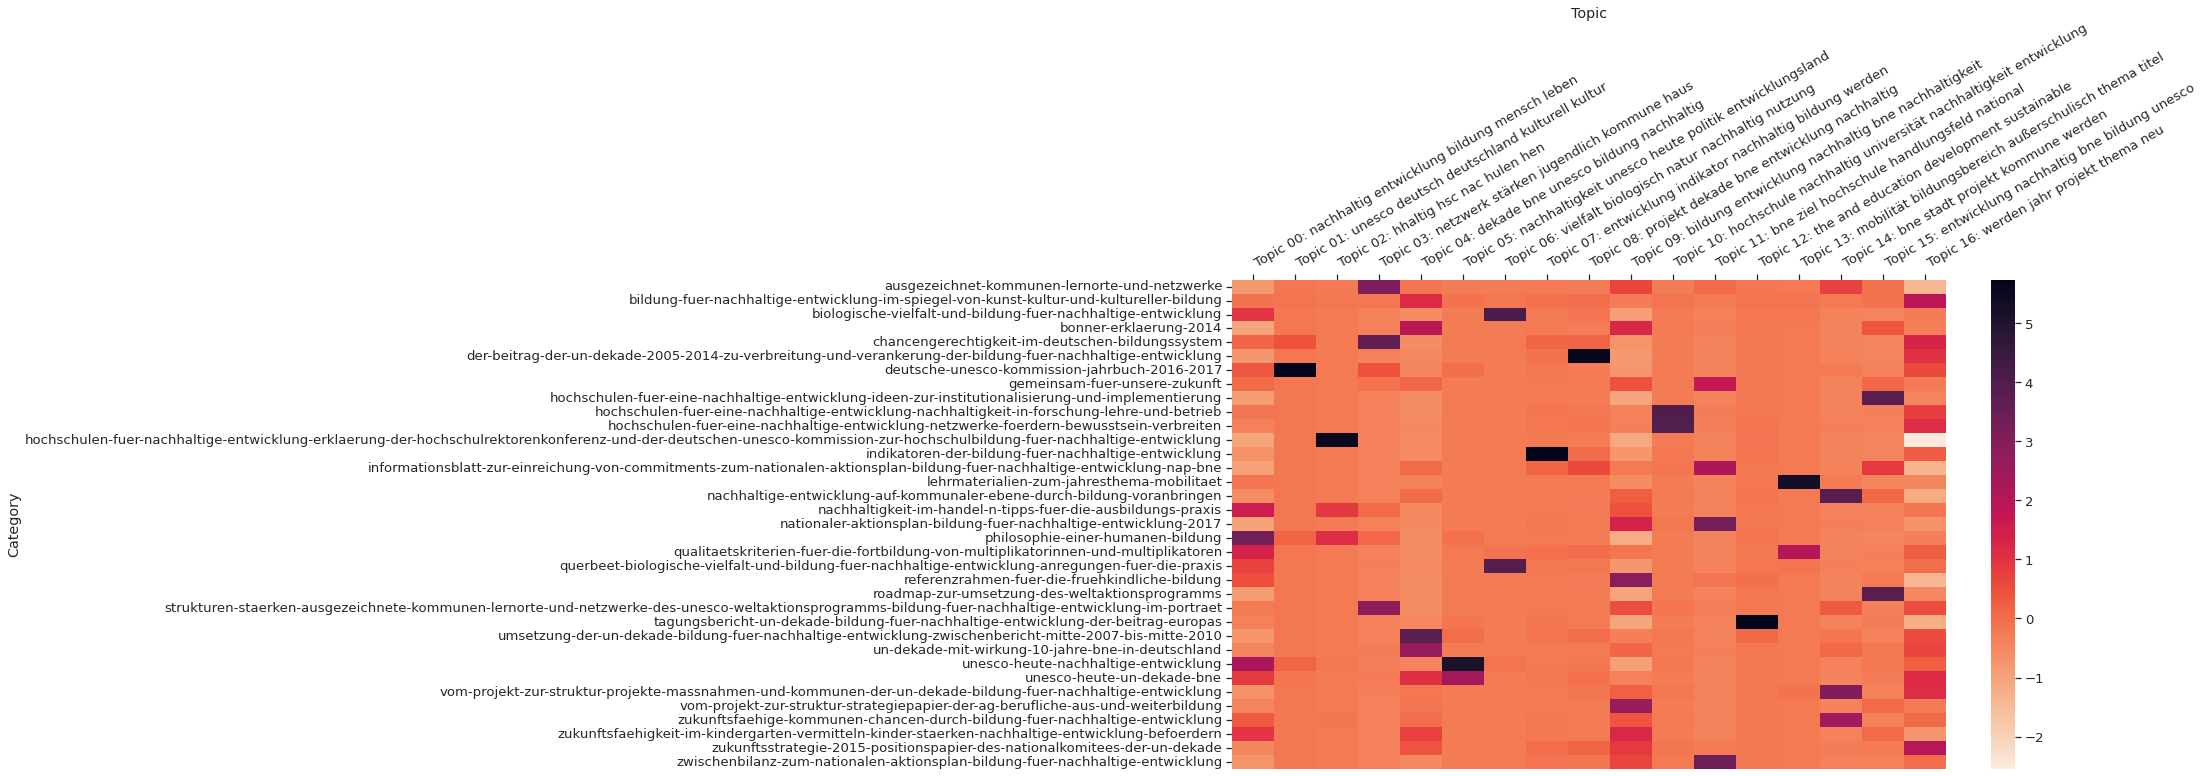
\includegraphics[width=1.0\textwidth]{img/Heatmap-BNE.png}\\
Es lassen sich hier die gleichen Ergebnisse wie in Kapitel 4.2 erkennen. Die Wahrscheinlichkeit, dass ein Topic in nur einem Text enthalten ist, ist bei Topic 1,2,7,8,12 und 13 sehr hoch, was durch die dunklen Flecken in der Heatmap dargestellt wird. Genau diese Topics wurden auch im vorherigen Kapitel identifiziert. Topics, die in mehreren Texten enthalten sind, zeichnen sich auf der Heatmap durch eine bunte Schattierung aus. Diese sind die Topics 0,4,9 und 16. Hier könnte vermutet werden, dass diese Topics inhaltlich ähnlich sind, da diese eine hohe Wahrscheinlichkeit haben in vielen Texten thematisiert zu werden. Solch eine thematische Überschneidung ist nicht zu erkennen. Die Wörter \textit{nachhaltig} und \textit{entwicklung} sind in einigen dieser Topics enthalten, was aber bei fast allen Topics zu beobachten ist. Durch die Darstellung der Heatmap ist eine dritte Kategorie erkennbar. Hierbei handelt es sich um Topics, die mit sehr hoher Wahrscheinlichkeit in zwei Texten zu finden sind. Das wird durch zwei lila Felder in einer Spalte sichtbar gemacht. Diese Topics sind Topic 3,5,6,10 und 15.

\subsection{Darstellung der Ergebnisse mit Blick auf den Inhalt der Topics}
Die vorliegenden Ergebnisse sind nicht so gehaltvoll wie erwartet. Die Topics sind nicht immer thematisch einheitlich und lassen sich oft nicht eindeutig zu einem der 17 SDGs zuordnen. Die Topics sind größtenteils dem SDG 4 \textit{Hochwertige Bildung} zuzuordnen. Dies ist angesichts der Herkunft der Texte nicht wirklich verwunderlich. Immerhin stammen diese aus dem Forum Bildung für nachhaltige Entwicklung. Das die meisten Texte demnach inhaltlich durch das Thema Bildung bestimmt werden ist demnach nicht verwunderlich. Die anderen Topics, die sich im weitesten Sinne mit einem der SDGs in Verbindung bringen lassen, sind die SDGs 11 \textit{Nachhaltige Städte und Gemeinden}, 8 \textit{Menschenwürdige Arbeit und Wirtschaftswachstum}, 15 \textit{Leben an Land} und 17 \textit{Partnerschaften zur Erreichung der Ziele}. Diese SDGs stehen auch in Verbindung zu den Themen Klimaschutz, Umweltschutz und Nachhaltigkeit. Auch wenn sich nicht alle Topics einem SDG zuordnen lassen, enthalten doch elf von 17 Topics das Wort \textit{nachhaltig}, neun Topics enthalten das Wort \textit{bildung} und acht das Wort \textit{entwicklung} - ein weiterer Verweis auf die Herkunft der Texte. Gar nicht werden hingegen humanitäre Themen wie die Bekämpfung von Hunger und Armut, Geschlechtergerechtigkeit und Frieden erwähnt. Interessant ist auch, dass das Topic 16 der BNE-Analyse. Hier erscheinen nur englische Wörter, was entweder darauf hindeuten könnte, dass ein englischer Text in dem Korpus enthalten ist, oder alle englischen Zitate gruppiert wurden. Zusammenfassend lässt sich über das Topic Modeling des BNE-Korpus sagen, dass sich einige SDGs ausmachen lassen, aber nur jene, die einen Bezug zu Bildung im Bereich Nachhaltigkeitsthemen haben. 

\subsection{Interessante Topics}
Einzelne Topics zeichnen sich durch Auffälligkeiten aus, was einer genaueren Untersuchung bedarf. Inhaltlich wie formell sind besonders die Topics 1,2 und 12 interessant.

\subsubsection{Genauere Betrachtung zu Topic 1}
In dieser Grafik lässt sich bei genauerem Betrachten einiges über die Texte aussagen. Das Topic 1 dürfte zum größten Teil aus dem Text \textit{Deutsche UNESCO Kommission Jahrbuch 2016-2017"}heraus entstanden sein. Tatsächlich enthält auch das Topic die Wörter \textit{deutsch}, \textit{deutschland} und \textit{unesco}. Thematisch zeigt das Topic auffällig viele Worte, die im Zusammenhang mit Kultur stehen. Ein Blick in den Inhalt des Textes macht deutlich, dass dieser Text Bildung im Bereich des kulturellen Erbes thematisiert. 

\subsubsection{Genauere Betrachtung zu Topic 2}
Bei der Interpretation von Topic 2 fällt auf, dass mit den Daten etwas nicht stimmen kann. 
Die höchste Wahrscheinlichkeit dieses krude Topic zwei zu enthalten, weist mit einem Wert von 0,958 der Text \textit{Hochschulen für nachhaltige Entwicklung Erklärung der Hochschulrektorenkonferenz und der deutschen UNESCO Kommission zur Hochschulbildung für nachhaltige Entwicklung} auf. Ein kurzer Blick in die Textdatei zeigt, dass diese unter der Umwandlung von pdf in txt gelitten hat und im Falle einer weiteren Arbeit mit diesen Texten weggelassen oder anders formatiert werden muss.

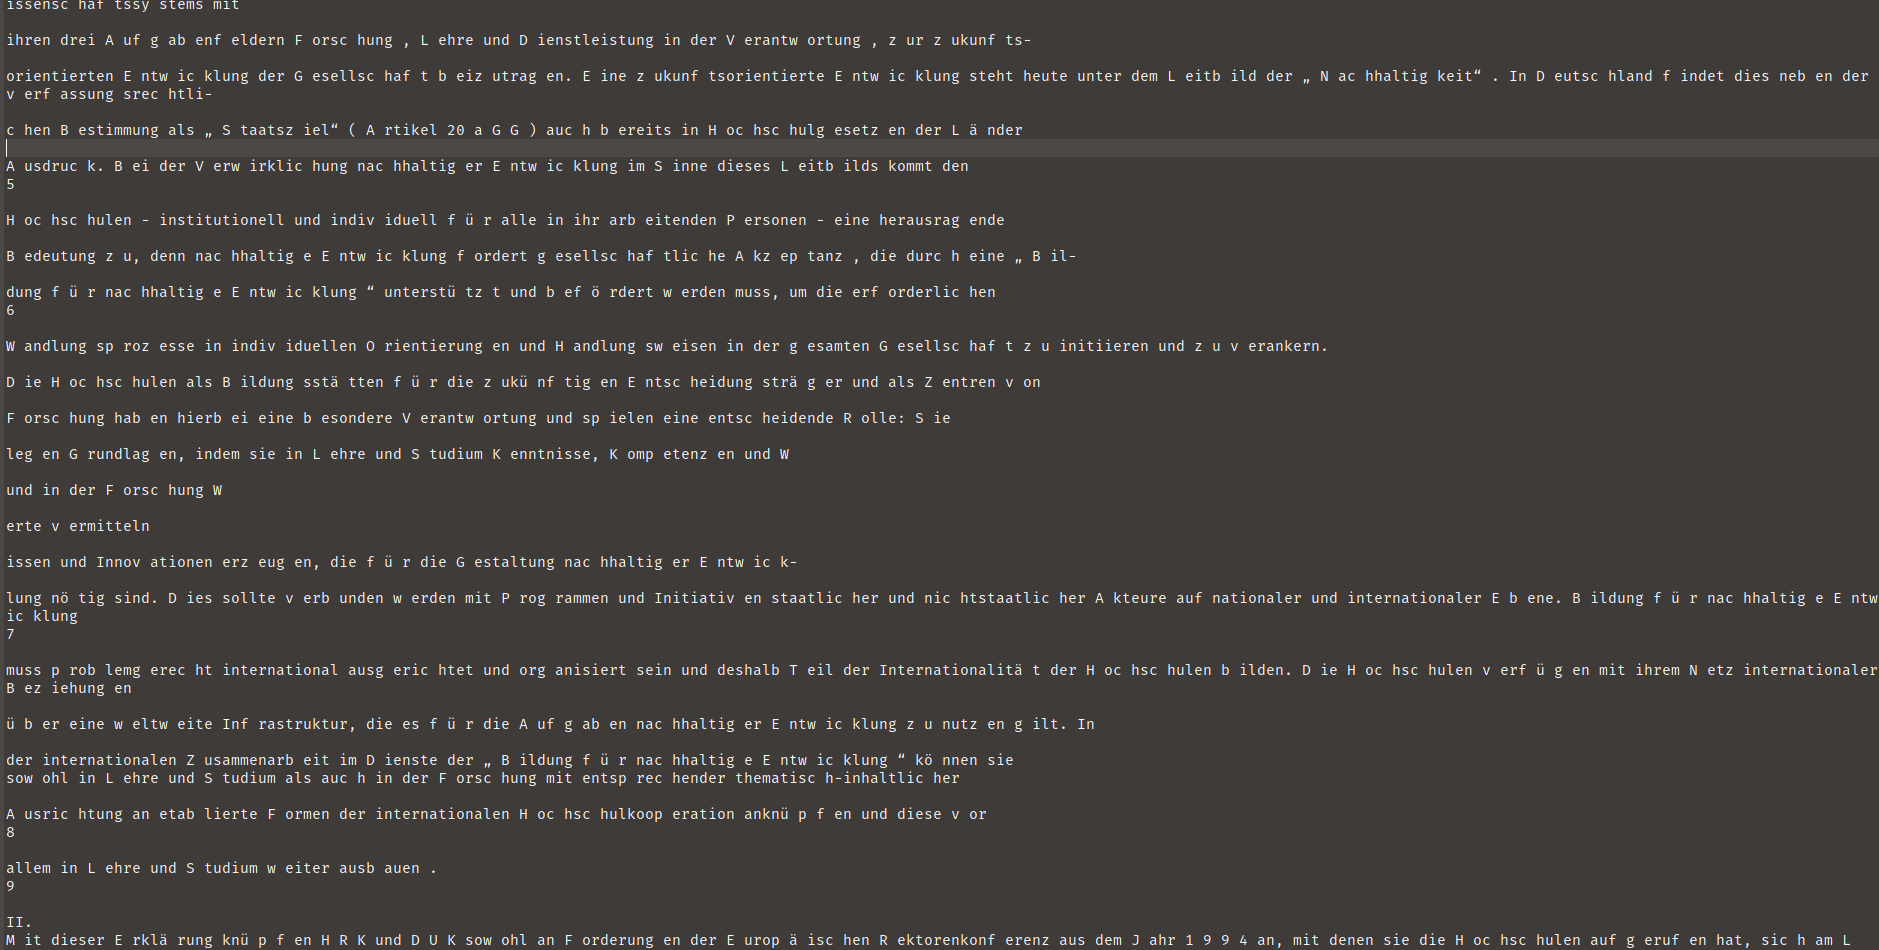
\includegraphics[width=1.0\textwidth]{img/Diffuser-text-Topic2.png}

\subsubsection{Genauere Betrachtung zu Topic 12}
Bei Topic 12 sind mehrere Besonderheiten erkennbar. Zum einen sind fast nur englische Worte enthalten, was darauf schließen lässt, dass sich ein englischer Text in den Korpus eingeschlichen hat. Die deutschen Worte, die jedoch enthalten sind, sind genau die Schlagworte, die den Korpus ausmachen: \textit{bildung}, \textit{nachhaltig} und \textit{entwicklung}. Die Vermutung liegt nahe, dass dieses Topic ganz besonders von einem Text beherrscht wird. Das Topic wird zu 73 Prozent in dem Text \textit{Tagungsbericht UN Dekade Bildung für nachhaltige Entwicklung der Beitrag Europas} erwähnt. Ein Blick in die Textdatei zeigt, dass dieser auf den ersten 60 Seiten auf Deutsch veröffentlicht und in der zweiten Hälfte auf Englisch veröffentlicht ist. Für eine weitere Analyse sollte dieser Teil aus dem Datensatz entfernt werden. 
\clearpage

\section{Fazit}
Nach Interpretation der Ergebnisse lässt sich sagen, dass die zu Anfang geplante Strategie mittels Topic Modeling von 17 Topics ein gutes Matching mit den SDGs zu erhalten nicht aufgegangen ist. Die Topics unterscheiden sich nicht sehr stark voneinander und eine Zuordnung zu einem der SDGs ist nicht so eindeutig wie erhofft.\\
Prinzipiell ist die Methode des Topic Modeling für so große Mengen an Texten, wie in der beschriebenen Analyse ein probates Mittel. Vielleicht hätte sich ein gelabeltes LDA Modell, das gleich auch die Überschriften zu den Topic generiert besser bewährt, um die Zuordnung zu den Topics nicht vom Ermessen des/der Autor*in abhängig zu machen. Jedoch lässt sich in dieser rein quantitativen Untersuchung der Texte erkennen, dass die Texte des BNE hauptsächlich das thematisieren, was sie thematisieren sollen. Das ist letztendlich Bildung im Bereich Nachhaltigkeit in verschiedenen Formen an Individuen weiterzugeben. Da das SDG 4 zugleich Ziel und Methode ist, die anderen SDGs zu erreichen, ist sein hoher Stellenwert in den untersuchten Texten logische Konsequenz. Zudem ist das Ziel von BNE nicht ausgewiesener Maßen die gleichberechtigte Thematisierung aller SGDs, sondern die besondere Stärkung und Verwirklichung des SDG 4 als Ausgangspunkt für die anderen Sustainable Development Goals. BNE verfehlt also nicht die Ziele der nachhaltigen Entwicklung, im Gegenteil, sie trägt durch die Umsetzung des Schlüsselziels der Bildung zu einem Erreichen der Ziele bei. Denn nur was auch verstanden wird, kann auch umgesetzt werden.\\
Abschließend bleibt noch darauf hinzuweisen, dass das strukturelle Problem der SDGs weiterhin bestehen bleibt. Auch wenn die hochgesteckten Ziele der SDGs als radikal und nie dagewesen gelobt werden, bezeichnet Aram Ziai in einem Artikel die SDGs als \glqq Trostpflaster eines Ungleichheit produzierendes globalen Kapitalismus\grqq{}. Ja, durch die ehrgeizigen Ziele der SDG wurden gerade in China und anderen Ländern des globalen Südens ein erfolgreicher Kampf gegen die Armut geführt. Jedoch lassen sich diese Erfolge nur unter einem postkolonialistischen Standpunkt feiern. Unter diesem kann Reichtum nur unter der Prämisse von Aneignung billiger Rohstoffe, Zerstörung von Ökosystemen und nicht-erneuerbarer Ressourcen fußen. Um eine wie eingangs beschriebene sozial, ökonomisch und ökologisch gerechte Welt zu erlangen, müsste eine Veränderung hin zu einem Gesellschaftsmodell vollzogen werden, die nicht auf dem althergebrachten Verständnis von Reichtum basiert\cite{Ziai}. Auch, wenn die SDGs ein guter und ehrenvoller Anfang sind, den zumeist menschengemachten Problemen der Menschheit entgegenzuwirken, bleibt doch fraglich, ob dies unter den bisherigen Rahmenbedingungen gelingen kann und sollte.

\clearpage

\begin{thebibliography}{xxx}
    \bibitem{BMZ} Bundesministerium für wirtschaftliche Zusammenarbeit und Entwicklung; zuletzt aufgerufen am 20.10.2021
        \url{https://www.bmz.de/de/service/lexikon/mdg-millenniumsentwicklungsziele-mdgs-14674}
        
    \bibitem{UN} Millenniums-Entwicklungsziele Bericht 2015, Vereinte Nationen 
        \url{https://www.un.org/Depts/german/millennium/MDG\%Report\%202015\%20German.pdf}
        
    \bibitem{Agenda2030} Bundesministerium für wirtschaftliche Zusammenarbeit und Entwicklung, Agenda 2030, zuletzt aufgerufen am 28.10.2021
        \url{https://www.bmz.de/de/agenda-2030/sdg-17}
        
    \bibitem{Bericht} Freiwilliger Staatenbericht Deutschlands zum Hochrangigen Politischen Forum für Nachhaltige Entwicklung 2021; Die Bundesregierung; Juni 2021
        \url{https://www.bmz.de/resource/blob/86824/6631843da2eb297d849b03d883140fb7/staatenbericht-deutschlands-zum-hlpf-2021.PDF}
        
    \bibitem{Ziai} Ziai, Aram. "Die SDGs–Eine postkoloniale Weinprobe." Entwicklungspolitik in Zeiten der SDGs. Essays zum 80 (2018): 205-209
    
    \bibitem{Bundestag} 
        \url{https://www.bundestag.de/services/opendata}
        
    \bibitem{OpenDiscourse} Richter, F.; Koch, P.; Franke, O.; Kraus, J.; Kuruc, F.; Thiem, A.; Högerl, J.; Heine, S.; Schöps, K. (2020). Open Discourse.  Harvard Dataverse. V3.
        \url{https://doi.org/10.7910/DVN/FIKIBO.}
        
    \bibitem{BNE} Bundesministerium für Bildung und Forschung; zuletzt aufgerufen am 28.10.2021
        \url{https://www.bne-portal.de/bne/de/einstieg/was-ist-bne/was-ist-bne_node.html}
        
    \bibitem{Moretti} Moretti, F. (2013). Distant Reading. London: Verso. 
    
    \bibitem{MALLET} McCallum, Andrew Kachites.  "MALLET: A Machine Learning for Language Toolkit."
        \url{http://mallet.cs.umass.edu. 2002.}
    
    \bibitem{MALLET_WELSH} zuletzt aufgerufen am 28.10.2021   
        \url{https://melaniewalsh.github.io/Intro-Cultural-Analytics/05-Text-Analysis/07-Topic-Modeling-Set-Up.html}
        
    \bibitem{LDA} Blei, David M., Andrew Y. Ng, and Michael I. Jordan. "Latent dirichlet allocation." the Journal of machine Learning research 3 (2003): 993-1022.
    
    \bibitem{Ramage} Ramage, Daniel, et al. "Topic modeling for the social sciences." NIPS 2009 workshop on applications for topic models: text and beyond. Vol. 5. 2009.
    
    \bibitem{ESD} United Nations Development Fund for Women (UNIFEM), "Education for Sustainable Development Goals. Learning Objectives", 2017, ISBN: 978-92-3-100209-0
        \url{https://www.bne-portal.de/bne/shareddocs/downloads/files/unesco_education_for_sustainab-ment_goals_learning_objectives.pdf?__blob=publicationFile&v=1}
    
    \bibitem{Zwischenbericht} Nationale Plattform Bildung für nachhaltige Entwicklung, "Zwischenbilanz zum Aktionsplan Bildung für Nachhaltige Entwicklung", Mai 2020
        \url{https://www.bne-portal.de/bne/shareddocs/downloads/files/zwischenbilanzhttps://www.overleaf.com/project/61ffb7d0c3bb4cd0cd764cac_nap_bne_1.pdf?__blob=publicationFile&v=1}
   
    \bibitem{HanTa} Christian Wartena (2019). A Probabilistic Morphology Model for German Lemmatization. In: Proceedings of the 15th Conference on Natural Language Processing (KONVENS 2019): Long Papers. Pp. 40-49, Erlangen.
    
    \bibitem{Agenda21} AGENDA 21, Konferenz der Vereinten Nationen für Umwelt und Entwicklung, Rio de Janeiro, 1992
        \url{https://www.un.org/depts/german/conf/agenda21/agenda_21.pdf}
    
    \bibitem{G} Geschäftsordnung der Nationalen Plattform Bildung für nachhaltige Entwicklung, 2021
        \url{https://www.bne-portal.de/bne/shareddocs/downloads/files/geschäftsordnung_NP_BNE.pdf?__blob=publicationFile&v=2}
        
    \bibitem{LDAorig} Blei, David M., Andrew Y. Ng, and Michael I. Jordan. "Latent dirichlet allocation." Journal of machine Learning research 3.Jan (2003): 993-1022.

\end{thebibliography}

\end{document}
